%--------------------------------------------------------------------------------------
% TDK paper
% Author: Donat Csikos
% Created at: 02.10.2012.
%--------------------------------------------------------------------------------------


%--------------------------------------------------------------------------------------
% Page format
%--------------------------------------------------------------------------------------
\documentclass[11pt,a4paper,oneside]{report}           
%\documentclass[11pt,a4paper,twoside,openright]{report}  


%--------------------------------------------------------------------------------------
% Package incudes
%--------------------------------------------------------------------------------------
\usepackage{t1enc}
\usepackage[utf8]{inputenc}
\usepackage{amsmath}
\usepackage{amssymb}
\usepackage{enumerate}
\usepackage[thmmarks]{ntheorem}
\usepackage{graphicx}
\usepackage{epsfig}
\usepackage{listings}
\usepackage{color}
\usepackage{lastpage}
\usepackage{anysize}
\usepackage{longtable}
\usepackage[english,magyar]{babel}
\usepackage{sectsty}
\usepackage{setspace}
\usepackage[hang]{caption}
\usepackage{subcaption}
\usepackage{hyperref}
\usepackage{tabularx}
\usepackage{palatino}
\usepackage{hyphenat}


%--------------------------------------------------------------------------------------
% Custom commands
%--------------------------------------------------------------------------------------
% insert pictures
\newcommand{\pic}[2]{
\begin{figure}[thb]
   \center   
   \caption{#2}
   \label{fig:#1}  
      \includegraphics{figures/#1}
\end{figure}
}

% insert and resize picture
\newcommand{\picr}[2]{ 
\begin{figure}[htb]
   \center   
   \caption{#2}
   \label{fig:#1}  
     \resizebox{\linewidth}{!}{
      \includegraphics{figures/#1}
      } 
\end{figure}
}


\newcommand{\secref}[1]{Section~\ref{#1}}                       % section reference
\newcommand{\code}[1]{{\upshape\ttfamily\scriptsize\indent #1}} % formatted code


%--------------------------------------------------------------------------------------
% Constant strings
%--------------------------------------------------------------------------------------
\newcommand{\pauthor}{Donát Csikós}
\newcommand{\psvisor}{dr.~István Ráth, Ákos Horváth}
\newcommand{\ptitle}{Incremental dependency analysis over large software infrastructure}
\newcommand{\pdep}{Department of Measurement and Information Systems}
\newcommand{\ptype}{}


%--------------------------------------------------------------------------------------
% Declarations
%--------------------------------------------------------------------------------------
\DeclareMathOperator*{\argmax}{arg\,max}
%\DeclareMathOperator*[1]{\floor}{arg\,max}
\DeclareMathOperator{\sign}{sgn}
\DeclareMathOperator{\rot}{rot}
\definecolor{lightgray}{rgb}{0.95,0.95,0.95}

\author{\pauthor}
\title{\ptitle}
\includeonly{
	title,%
	chapter1, chapter2, chapter3, chapter4, chapter5, chapter6%
}

%--------------------------------------------------------------------------------------
% Page layout setup
%--------------------------------------------------------------------------------------
% we need to redefine the pagestyle plain
% another possibility is to use the body of this command without \fancypagestyle
% and use \pagestyle{fancy} but in that case the special pages
% (like the ToC, the References, and the Chapter pages)remain in plane style

\pagestyle{plain}
%\setlength{\parindent}{0pt}                  % more clear; in english documents
%\setlength{\parskip}{8pt plus 3pt minus 3pt} % more clear; in english documents
\setlength{\parindent}{12pt}                  % in hungarian documents
\setlength{\parskip}{0pt}                     % in hungarian documents
\marginsize{35mm}{25mm}{15mm}{15mm}           % anysize package
\setcounter{secnumdepth}{0}
\sectionfont{\large\upshape\bfseries}
\setcounter{secnumdepth}{2}
\singlespacing
\frenchspacing


%--------------------------------------------------------------------------------------
%	Setup hyperref package
%--------------------------------------------------------------------------------------
\hypersetup{
    %bookmarks=true,           % show bookmarks bar?
    unicode=false,             % non-Latin characters in Acrobat’s bookmarks
    pdftitle={\ptitle},        % title
    pdfauthor={\pauthor},      % author
    pdfsubject={\ptype},       % subject of the document
    pdfcreator={\pauthor},     % creator of the document
    pdfproducer={Producer},    % producer of the document
    pdfkeywords={keywords},    % list of keywords
    pdfnewwindow=true,         % links in new window
    colorlinks=true,           % false: boxed links; true: colored links
    linkcolor=black,           % color of internal links
    citecolor=black,           % color of links to bibliography
    filecolor=black,           % color of file links
    urlcolor=black             % color of external links
}


%--------------------------------------------------------------------------------------
% Set up listings
%--------------------------------------------------------------------------------------
\lstset{
	basicstyle=\scriptsize\ttfamily,              % print whole listing small
	keywordstyle=\color{black}\bfseries\underbar, % underlined bold black keywords
	identifierstyle=, 					          % nothing happens
	commentstyle=\color{white},                   % white comments
	stringstyle=\scriptsize\sffamily, 			  % typewriter type for strings
	showstringspaces=false,                       % no special string spaces
	aboveskip=3pt,
	belowskip=3pt,
	columns=fixed,
	backgroundcolor=\color{lightgray},
} 		
\def\lstlistingname{lista}	


%--------------------------------------------------------------------------------------
% Setup captions
%--------------------------------------------------------------------------------------
\captionsetup[figure]{
%labelsep=none,
%font={footnotesize,it},
%justification=justified,
width=.75\textwidth,
aboveskip=10pt}

\renewcommand{\captionlabelfont}{\small\bf}
\renewcommand{\captionfont}{\footnotesize\it}


%--------------------------------------------------------------------------------------
% Main document content
%--------------------------------------------------------------------------------------
\begin{document}

\pagenumbering{arabic}
\onehalfspacing


\selectlanguage{english}
%--------------------------------------------------------------------------------------
%	The title page
%--------------------------------------------------------------------------------------
\begin{titlepage}
\begin{center}
%\includegraphics[width=60mm,keepaspectratio]{figures/BMElogo.png}\\

\includegraphics[width=60mm,keepaspectratio]{figures/BME1782nagy.pdf}\\
\vspace{0.3cm}
\textbf{Budapest University of Technology and Economics}\\
\textmd{Faculty of Electrical Engineering and Informatics}\\
\textmd{\pdep}\\[5cm]

\vspace{0.4cm}
{\huge \bfseries \ptitle}\\[0.8cm]
\vspace{0.5cm}
\textsc{\Large \ptype}\\[4cm]

\begin{tabular}{cc}
 \makebox[7cm]{\emph{Author}} & \makebox[7cm]{\emph{Supervisors}} \\
 \makebox[7cm]{\pauthor} & \makebox[7cm]{\psvisor}
\end{tabular}

\vfill
{\large \today}
\end{center}
\end{titlepage}




\tableofcontents

\chapter{Introduction}
% ------------------------------------------------------------------------------
% 2 pages. give a short overview about the environment and introduce the problem
% what my solution solves.
% ------------------------------------------------------------------------------

\section{Motivation}

In today's software development practice, large projects that involve many
interrelated software components are a commonality. To tackle the complexity of
such development processes, a primary aim for both project managers and
developers is to reduce inconsistency issues that may arise due to the
combination of (i) development by large and distributed teams and (ii) the
complex dependency relationships within the system under development.

In a Java context, a typical example of such problems is when a newer
version of some component is binary incompatible with others that depend on
(link to) it. Even though linking errors can be detected at compile time in
theory, in practice this may not be always feasible as the entire source tree
may not be available to every developer.

The main challenge addressed in this work is to achieve \emph{smooth upgrades}~\cite{Ical11}.
A smooth upgrade means that after a new version of a software component has been
released, all the other software components which depend on it will remain
operational.

There are a variety of approaches and tools to support smooth upgrades. For
instance, one can enforce development process policies that involve manual
synchronization steps that all developers must follow. An alternative approach
-- perhaps better aligned with agile principles -- is to provide automated tools that
relieve the developers of the difficulties associated with software
infrastructure management.

In this work, we aim to develop such an automated tool based on static
\emph{dependency analysis}. In a few words, the goal of the tool is to assist
developers in situations such as when e.g. a bug needs to be fixed which
requires a change in a library API.
In this case, the tool should help the developer in checking which other
components are using that API, more specifically which parts of the API are
being used, which functions should remain untouched and which can be changed
freely. Using information provided by the tool, the developer should be able to
resolve such issues on her own, or in the worst case know exactly which other
team members are to be notified and called in for assistance.
 
\subsection{Controls Systems at CERN}
The context of this work is the author's internship at the Controls Group of
CERN, the European Organization for Nuclear Research. CERN runs the world's
biggest particle physics laboratory with the main goal to operate particle
accelerators (such as the Large Hadron Collider) and all the necessary
infrastructure. At CERN, numerous scientist and engineers are working on the
design and the maintenance of the software and hardware equipment in a
well-defined structure. One of its members is the \emph{Controls Group} which is
responsible for the design and implementation of both software and hardware used
in the controls systems.

The controls systems themselves are complex, distributed and highly modular systems
with three main tiers. On the top there are the GUI applications which are
written in Java. The middle or business layer is also consists of Java
applications. On the lowest or hardware level there are C/C++ applications
running on real-time systems. Maintaining a complex system like this requires a
set of special approaches in order to provide desired quality and to maximize
the availability of the systems. The primary objective for the Controls Group is
to maintain uninterrupted operation without any downtime. During the internship,
the author was tasked with designing and implementing a developer tool that
should aid the software developers at CERN in minimizing software component
upgrade problems.

\subsection{Requirements specific to the deployment environment}
There are certain requirements specific to the software infrastructure at CERN
that needed to be taken into consideration while designing the system.

\begin{description}
\item[Technological environment] The software components to be managed by the
new tool are all plain Java programs that do not make use of any framework (such
as OSGi) for dependency and lifecycle management, but rely on basic
features of the Java Compiler and the Java Virtual Machine to link to each
other.
 
\item[Complexity of a large software infrastructure] In a simple case,
dependency analysis could be supported by a development environment such as
Eclipse based on integrated source/binary code analysis. However, CERN Controls
Systems deals with an infrastructure that consists of several thousands
components (JARs) and even more if version information is taken into
consideration. The resources available for development environments at developer
PCs are not enough for supporting standard IDE features over a system of this
size.
 
\item[Granularity of dependencies] Existing dedicated dependency analysis
tools offer a rat\-her limited feature set for defining dependency relationships.
For example JDepend \cite{JDepend} and JBoss Tattletale \cite{Tattletale} does
dependency analysis on the class level, but CERN's requirement is to see
method-level and fields level dependencies as well.

\item[Source code analysis alone not feasible] Due to legacy reasons at CERN,
the (up-to-date) source code is not available for some software components. In
other cases, the source code is very large in size because it is automatically
generated. Therefore, tools that rely solely on source code analysis cannot be
used.

\end{description}

\section{Overview of the proposed solution}
After analyzing available off-the-shelf solutions, it became clear that the
unique requirements called for a custom solution. The result of the work called
\ptool{} implements hybrid dependency analysis based on both source and binary
software components and relies on a client-server architecture where end-user
features are specifically aligned with the computing resources of the host
environment. The tool uses a state-of-the-art incremental model query evaluation
engine called EMF-IncQuery (developed at the Department of Measurement and
Information Systems of the Budapest University of Technology and Economics), to
provide on-the-fly dependency analysis results integrated into the Eclipse
development tool.

\subsection{Server features}
On the server side, the \ptool{} provides the following features:
\begin{itemize}
  \item \emph{Binary dependency discovery based on byte code analysis} ensures
  that all (including legacy) software components can be taken into
  consideration for smooth upgrades, at the desired level of granularity.
  \item A \emph{scalable relational dependency database} back-end ensures that
  the entire, large software infrastructure can be supported.
  \item A \emph{data access layer based on Java RMI} allows accessing dependency
  data by Java-based clients in an efficient way.
\end{itemize}

\subsection{Client features}
On the client side, the \ptool{} provides the following features:
\begin{itemize}
  \item Efficient \emph{source dependency discovery based on incremental AST
  processing}, supported by the Eclipse Java Development Tools.
  \item A \emph{model-based dependency representation for both local (source)
  and remote (binary) dependencies} based on the Eclipse Modeling Framework. The
  industry standard modeling format allows the processing of dependency data by
  third party modeling tools.
  \item \emph{On-the-fly dependency queries based on the joined local and remote
  dependency model} supported by EMF-IncQuery. As the dependency queries are
  evaluated very efficiently, the system is able to provide instantaneous
  dependency analysis feedback (relevant to both local and server-side
  information) as the source code is being changed by the developer.
  \item \emph{User interface integration components for both client-side and
  server-side queries} that allow ease of use for developers accustomed to the
  Eclipse environment.
\end{itemize}

\section{Structure of the report}
The rest of this report is structured as follows. Chapter 2 gives a brief
overview of technologies that have been used in the design and implementation.
Chapter 3 discusses the role of the tool in development workflow (Section 3.1),
provides a high-level overview of the software system architecture (Section 3.2)
and introduces a running example that is used in explanations later on (Section
3.3). Chapter 4 elaborates the design and implementation details, by discussing
components both on the server side (Section 4.1) and client side (Section 4.2).
Chapter 5 presents experimental results on the performance evaluation of the
system, and Chapter 6 concludes the report with discussing on future work.

%\todo[inline]{change for proper refs}



\chapter{Background}
%------------------------------------------------------------------------------
%10 pages. For motivation: Design pattern figure. (Service registration pattern).
%------------------------------------------------------------------------------


\section{Related technologies}
% Why do we need this part.
Before proceeding to the main part of this paper, I am going to give an overview
about the related technologies used by my solution. I Why do we have to present
the related technologies.

\subsection{Java Runtime}

\subsubsection{Java byte code specification}
How the java vm works.
What is the input.
What kind of information can be extracted from here.

\subsubsection{Apache Commons Byte Code Engineering Library}
% described in the virtual machine specification 
% http://docs.oracle.com/javase/specs/jvms/se5.0/html/VMSpecTOC.doc.html 
% how the virtual machine works
% what kind of infomration is available in the bytecode 
\cite{BCEL}
Abstraction over Java byte code specification. 
How it works. Create diagram!
Possible use-cases.


\subsection{Eclipse}

\subsubsection{Eclipse Integrated Development Environment}
The Eclipse Project \cite{Eclipseproject} is an open source software development
project dedicated to providing a robust, full-featured, commercial-quality,
industry platform for the development of highly integrated tools. It was
developed by IBM from 1999, and a few months after the first version was
shipped, IBM donated the source code to the Eclipse Foundation.

The Eclipse project consists of many subprojects, the most important being the
Eclipse Platform, that defines the set of frameworks and common services that
collectively make up ,,integration-ware'' required to support a comprehensive
tool integration platform. These services and frameworks represent the common
facilities required by most tool builders, including a standard workbench user
interface and project model for managing resources, portable native widget and
user interface libraries, automatic resource delta management for incremental
compilers and builders, language-independent debug infrastructure, and
infrastructure for distributed multi-user versioned resource management.

The Eclipse Platform has an easily-extendable modular architecture, where all
functionality is achieved by plugins, running over a low-level core called
Platform Runtime. This runtime core is only responsible for loading and
connecting the available plugins, every other functionality, such as the
editors, views, project management, is handled by plugins. The plugins bundled
with Eclipse Platform include general user interface components, a common help
system for all Eclipse components, project management and team work support.

\subsubsection{Eclipse Java Development Tools}
% TODO: Write jdt description with the same details as the Eclipse platform.

\subsubsection{Eclipse Modeling Framework}

\subsubsection{EMF-IncQuery} 
Incremental model queries over emf models. Documentation site.
% https://viatra.inf.mit.bme.hu/incquery/documentation

\subsection{Other related technologies}

\subsubsection{Spring Framework}
To develop modular, testable and configurable applications.
\subsubsection{Maven}
Build system
\subsubsection{Tycho}
Maven extension to build eclipse plugins.
\subsubsection{Oracle database}
Commercial relational database management system. Full sql support. Extensive
feature set, one of the market-leaders.
% maybe it is easy to put here something from wikipedia.


\section{Example: Service Provider Framework}
\label{sect:example}

The service provider framework is a possible use-case for the Adapter design
pattern. The implementation I am going to present derived from the book
\cite{Bloch08} Effective Java.

Overview of the pattern. 
\picr{exampleclasses.pdf}{Service Provider framework example}
Three different people 

Description of the classes one-by one. Possible source code can be inserted
here.

% ------------------------------------------------------------------------------
% 3 pages. Super figure which describes the entire solution. Choosing proper
% abstraction level for the %figure is essential. Every item on this figure will
% be an additional chapter in this paper.
% TODO:find a proper name for this chapter.
% ------------------------------------------------------------------------------
\chapter{Overview}


\section{Architecture}
% My implementation.
As it was discussed previously one of the most effective  way of achieving
smooth upgrades is to discover incoming dependencies. For this I designed and
implemented a solution called \ptool{}. \picr{superfigure.pdf}{Overview of the
implemented system} \autoref{fig:superfigure.pdf} shows the overview of
it.

% Two implementation
This systems was implemented in two separate steps. My work at CERN covered an
implementation of a system which gives the ability to the users to query certain
parts of the source code for incoming dependencies. After my job was done I
created an extension which utilizes EMF-IncQuery to run faster, information-rich
and more extensive queries. Let's examine the elements of the figure one-by-one.


\subsection{System boundaries}
The system allows the users to examine the inter-project dependencies from the
development environment. It exposes two access points to access this
information. First the developer can initiate queries explicitly by selection
the target element from  he source code editor. The other option to check result
of the model queries (described later). This information is updated
automatically, every change in the development environment is reflected to the
result set. Both versions give visual representation of the result which the
developer can analyse and he can use it to make decisions what to and what not
to change in the source code.


\subsection{Repository management}
% Central repository management.
The first elements on the figure to discuss are the ''Source repository'' and
the 'Binary component repository' . They contain both the source code and the
build binary version of the internally developed softwares. These elements are
centrally managed and have a well-defined structure. The developers work on the
source code and if they finish one milestone they publish their improvements by
putting the compiled version into the binary repository through an automated
process.
The binary repository is the input for the dependency analysis.

\subsection{The server side}
The server side is a standalone Java application which runs on a Linux server.
It has two functionality: 1) it discovers and stores the structure of the
products and 2) provides an interface for serving dependency queries.

For discovering, the process listens if a new release happens in the repository.
If it happens the freshly added binaries (jar files) are passed to the byte code
analysis module which parses the file and discovers the contained structure and
the dependencies utilizing the Apache BCEL library.  The structure and the
dependencies are passed to the storage engine to store it. The storage engine
itself defines a set of operations to find, store and retrieve certain subset of
the model. The remote query interface also use this module to get the necessary
dependency information for the clients.


\subsection{The client side}
% Plugin
The client-side of the solution is an Eclipse plugin (or more precisely a set of
plugins) which gives the developer a convenient way to access to the dependency
information.

% Model load and direct queries
The base of the plugin is the repository model loader. It provides a simple API
for accessing and querying the dependency information from the server. The
simple use-case for this, when the user directly asks the dependency information
from the Java source editor through UI contribution (marked as direct queries on
the figure).

% ws model creator
The workspace model creator is module generating an EMF model describing the
state of the workspace. The generated model contains the loaded projects, the
contained packages, classes, methods, etc. The model also contains the
dependency structure between the elements (e.g. method calls, field accesses and
such). The information is gathered through the Eclipse Java Development Tools'
API. After the model is created it is incrementally maintained even through 
restarts.

% pattern maching over.
The pattern matcher module executes complex model queries on top of the acquired
models to provide dependency information. First it loads an EMF model from the
server describing the structure of all projects in the central repository.
Afterward the workspace model is loaded from the module described above. Both of
the models are loaded to the EMF-IncQuery engine. Through complex queries the two
models are joined and queried for the dependency information. With this more 
accurate and extensive dependency analysis can be achieved because this approach
takes into account the changes which were done in the workspace. The workspace 
model is updated upon every change of the workspace giving up-to-date feedback 
for the users while they are working on the development. 

% Interface.
Both direct queries and the pattern matching module return the result in Eclipse 
views. After the result is evaluated, the user's responsibility to evaluate their
results and act accordingly.

% limitation.
Using direct queries brings no limitations. The queries are simple remote method
calls and the result set is a relatively small data set which easy to store and
present on the Eclipse UI. On the other hand, the pattern matching solution is
far from being that easy, because in order to load make EMF-IncQuery work, the
entire repository has to be loaded. By default this model is a few hundred
megabytes sized in a serialized form. This implies that the implementation has to 
optimize this model without dropping useful information to make it loadable to 
the memory.

\section{Service Provider Framework}\label{sect:spf}

\subsection{Description of the pattern}

To make the following chapters easier to understand, I am going to introduce a
simple use-case example. It is a design pattern called Service Provider
Framework. It is a practical application of the original Adapter pattern and it
was described in the famous book ,,Effective Java'' \cite{Bloch08}. This pattern
is the simplified version how the Java Database Connectivity (JDBC) works.

\picr{exampleclasses.pdf}{Structure of Service Provider Framework pattern}

You can see the structure of the pattern on
\autoref{fig:exampleclasses.pdf}. As of the packages it contains 3 major parts.
The \code{service} package contains the core pattern classes. The \code{impl}
and the \code{impl} packages are external users of the pattern and therefore
they are considered depending client libraries.

First let's discuss the pattern itself. The main goal for the patter is to
provide a registry of implementations for a desired service. This service is
described in the \code{Service} interface. The \code{Provider} interface is
serves as a factory instance; it has a single function to instantiate a new
Service object. The \code{Services} class has the role of the registry.
The service implementers register their implementation using the static
\code{registerProvider()} and \code{registerDefaultProvider()} methods. The
parameters the identifier string for the registered service and Provider
instance which will instantiate the Service instances. The clients will
instantiate the Service instance with the \code{newInstance()} function.
Depending the passed identifier string, the method will look up if a Provider
was registered with the same name, and if the answer is yes then it calls the
\code{Provider.newInstance()} and return its result.

The \code{DEFAULT\_PROVIDER\_NAME} is a static public field which can be used to
obtain the default Service implementation. The \code{AbstractService} is a
utility class which implements one of the function of the Service interface.

The \code{impl} package contains one possible implementation to use the
described pattern. The \code{BasicService} contains the implementation and the
\code{BasicProvider} is responsible for properly initializing and returning a
new instance of this version. The \code{BasicImplUtil} -- as its name implies --
holds utility classes which register the implementation in the Services class.

The \code{client} package holds one single \code{Main} class, which contains a
simple evaluation. It invokes the \code{Services.newInstance()} function passing
the default provider's name as an argument and invokes the \code{serviceA()} and
\code{serviceB()} function.

Although the example is fairly simple, the related source code can be found in
\autoref{examplesource}.

\subsection{Description of the problem}
As it was described in the introduction we would like give the developers the
ability to check who is using the certain parts of the API. To present this this
pattern will be our use-case.

Imagine that the three packages are distributed into three different software
which have their individual developers. If somebody wants to change some parts
of the service without precisely knowing who is using which part of the code he
won't know how many dependant projects will be broken afterwards.

Let's see two examples. The responsible for the service package wants to modify
two parts of the classes: he wants to add a string parameter to the
\code{Service.serviceA()} method, and he wants to change the name of the
\code{Services.DEFAULT\_PROVIDER\_NAME} field. 

By using \ptool{} the developers are able to execute queries on any part of the
API. The result will be the primary starting point for considering what to do.
Three different outcome can happen: the selected part of the API doesn't have
dependencies, it has a few dependencies or it has got a lot and the developer's
decision depends on it. 

If there is no incoming dependency than any modifications can be done without
causing any compatibility issues. The developer can do whatever he wants.
If there is a lot of incoming dependency, than it means that the queried code
element is used by a lot of clients and any modifications would cause a build
error therefore backward compatibility has to be maintained. The third option is
that there are several dependencies. In this case the developer has to negotiate
with the clients how to proceed: he has to provide backward compatibility or the
clients has to align their code to the modifications.



\chapter{Details}
% ------------------------------------------------------------------------------
% Elaboration 20 pages. Details of the Dependency Analysis Plugin (DAP. Describe
% the DAP-DB and %DAP-INCQUERY solution too.
% ------------------------------------------------------------------------------


\section{Infrastructure at CERN controls systems}


\subsection{Used tools}
- Describe, how a typical developer works at CERN BE-CO - Tools: SVN, Eclipse,
Common Build, JIRA, etc. % check this at some papers of vito.


\subsection{Development workflow}
- Original idea comes from the typical development workflow lifecycle at CERN
control systems. %Insert one-by one the explanation form my thesis1 report.


% ------------------------------------------------------------------------------
% MODULE: Bytecode analysis
% ------------------------------------------------------------------------------
\section{Bytecode analyzer}
% Why
Before the system performs dependency analysis, it needs to extract the
necessary information from the source code.
% What
The Bytecode analyzer module takes the input java binaries (in the form of jar
files) parses the contained class files with the help of Apache BCEL and maps it
into an object graph which can be effectively used during the dependency
processing.


% How
\subsection{Anatomy of a Java binary}
The Bytecode analyzer module takes a set of jars as an input. A jar file is
essentially a zip file containing Java-related resources: resource files, binary
class files and meta-information. Because the system has to discover
dependencies between pure Java applications then no meta-information is used;
the bytecode analyzer gets the information from the class files contained in the
jars.


% Describe the ConstantMethodRef/FieldRef/Class/String in more details?
Figure \autoref{fig:classfile.pdf} shows a simplified view how a single class
file is built. This structure is precisely defined in Java Runtime
Specification. The class begins with a marker header followed by the part called
\textit{constant pool} which contains the textual part of the code. It contains
the i) constant strings ii) referenced methods and fields and iii) the names of
the external classes. The Java virtual machine is only able to load a class file
if all the referenced external classes are loaded.
\pic{classfile.pdf}{Internal structure of a class file}
After the constant pool the access flags, the implemented interfaces and the
field list are located in separate places.

% Describe the bytecode instructions?
Afterwards comes the definition of the methods. It contains all the necessary
information for the virtual machine to execute the methods: the resources to 
allocate for the execution, the exception handlers and the bytecode itself. 

The big question is what information can be extracted from the jar/class files
for the dependency analysis? The short answer is everything. The structure of a
class file can be obtained one-by-one. The external references what we are
looking for are also fairly easily to extract, because they are defined in the
constant pool. The only challenging part to solve is to match, where exactly are
the external resources are used in the bytecode itself.


\subsection{The analysis process}
The module extract all necessary information from the class files for processing
them. This could be done by brute-force parsing binary files, but it would be an
tedious and error-prone task. Instead of this the implementation reuses Apache
BCEL to effectively parse the class files and and to obtain the necessary
information via simple API calls.
\pic{bytecodeanal.pdf}{Steps of the bytecode analysis process}
\autoref{fig:bytecodeanal.pdf} shows the steps of the analysis process and the
related information in the class files for each step. 

The analysis starts with gathering the basic structure. This involves acquiring
the class' name, the name of the extended class and the implemented interfaces,
the defined fields and methods. This information is accessible out of the box
through the BCEL API.  

The second step is to acquire all external reference pointing outside of the
class files. For imported classes it is easy because this is what the
\code{ConstantClass} entries cover in the constant pool. For field and method
references, the implementations searches \code{ConstantFieldRef} and
\code{ConstantMethodRef} occurrences in the bytecode and saves all methods 
which uses them.

The next step is to convert the information into source format. This is
necessary because both the structure and the external references are presented
in a format which not readable nor could be easily queried by the users of the
data. For example the commonly used \code{println(String)} function has the
following binary format: \code{println(Ljava/lang/String;)V}. The implementation
transforms it into \code{println(java.lang.String):void}.

% Somewhere it should be described that we don't deal with reflection, just
% static dependencies.
The final step is to cleanup the gathered information. At this step have to
consider that if we mapped all information then the gathered data would have a
comparable size with the binary repositories which is unacceptable when we have
to deal with thousands of jars. To resolve this, the implementation does
multiple cleanup steps. First it drops the private methods and fields, because
it is not explicitly accessible and by this no dependency would point them. The
other trick is to drop a subset of the external references. The
platform-provided elements are dropped (references pointing inside the
\code{java.*} package) and the ones which point inside the jar files. This is
reasonable because any IDE gives access this information through code traversal
capabilities. Of course this cleanup needs do be done after all class files are 
parsed in a jar file. 


\subsection{Extracted domain model}
The output of the analyzer is a java domain model.
\picr{domainmodelsimp.pdf}{Classes of the domain model used by the bytecode analyzer}
\autoref{fig:domainmodelsimp.pdf} shows the elements of this model. Because this
model is used for the dependency processing too the model has additional
elements which is now not important.

All element inherits from abstract \code{CodeElement} class which is a top-level
interface for handing the items of the model. The processed jar files are named
as \code{Product}s, because that's what it is: a software product. A product
contains several classes named \code{ApiClass} which store the class-level
properties. The required classes are stored in the \code{referencedClasses}
list. The classes contain some \code{Field}s and some \code{Method}s which both
have a -- source formatted -- signature and some access properties. The
\code{referencedFields} and the \code{referencedMethods} hold all the external
field and method references which are accessed or invoked in the bytecode of the
represented method.

With an instance of this domain model the dependency processing module is
capable of discovering the dependency relationships between certain parts of the
dependency.
 

% ------------------------------------------------------------------------------
% MODULE: Dependeney processor
% ------------------------------------------------------------------------------
\section{Dependency processor}
% Why
The bytecode analyzer gathers all structural elements and the textual references
of the dependencies. For resolving the references the dependency processor
component is responsible.

% What
To achieve this the processor takes the models of the jar files, compares the
contained references with the structure of the external jars. When a match is
found it means that there is a dependency between a two elements and as a result
a dependency is stored.

% How
\subsection{Discovered dependencies}
During the work at CERN we decided to narrow down the search for basic
dependencies which could be extracted from the binary code without interpreting
what does a class really do. By this we could exactly define what information
will be accessible for the users. The following list contains the discovered
dependencies:
\begin{description}
\item[Class import] When a class uses \emph{any} part of an external class. 
Practically this is a relationship between two classes when one class requires
the other to get loaded in the Java virtual machine. On a binary level it is 
expressed as a \code{ConstantClass} entry in the constant pool.  
\item[Inheritance] When a class inherits from another. This dependency type 
covers both the case when an interface is implemented and when a class is 
extended. 
\item[Method call] When a method calls an another method. Covers both static 
and non-static method calls.
\item[Method override] When a class extends from an another and the subclass 
has a method with a same signature which was already defined in the superclass.  
\item[Field access] When a method accesses or gives a value of a field defined 
in an external class.
\end{description}


\subsection{Discovery process}
After defining the searched dependencies let's see how exactly the dependency
discovery process work. The main objective here is to do the analysis on a large
set of Java binaries without having memory problems. Obviously if one loads all
jars at the same to the memory and searches for all references it will need an
enormous size of memory which will go up if the input number of the binaries
increasing.

\picr{analization.pdf}{Sequence of the dependency discovery process}
\autoref{fig:analization.pdf} shows how the tool solves this issue. The process
starts with an update in the binary repository. The new, not analyzed binaries
are passed to the bytecode analyzer components which produces a model for each
jar files. These models passed for the dependency processor which stores the jar
structure in the database. By doing this the implementation holds only one model
in the memory which implies that the memory requirement is independent from the
number of input binaries. Also only the structure is pushed into the database,
the references are considered as transient data. This is necessary because the
references need huge space to store: on average they took 60\% of the size of a
class file and leaving them out is a big saving in the storage.
 
After all jar's  structure is saved in the database, the process re-initiates
the bytecode analysis on every jars one-by one and passes the models again to
the dependency processor. The processor now tries to execute certain queries on
the database for searching dependencies. For external references it tries to
find the elements with the same fully qualified, for inheritance searches for
superclass in the database and for method override it looks for methods with
the same signature in the superclass. Every found element from the database 
result in a dependency entry at the end of the analysis of the current jar. 

The result of the analysis is a database containing all the structure
and the dependency information. The clients execute queries on it to analyze the
relationships between certain elements in order to decide whether or not a
specific code could be changed.
 
\section{Storage engine} 

The dependency processing requires requires some database functionality to 
properly work. This is defined in the storage engine component.

Although this component is defined by a single Java interface it comes with
important and complex responsibilities. First it is an abstraction layer over
the concrete database implementation. Second it provides transactional behaviour
automatically to the database. 

The interface defines operations for two purposes: i) Store and retrieve the
structure of a jar and the dependencies ii) search for items based on their
names and iii) query incoming dependencies of an element.

The usage of the first is easy the understand: if the analyze process starts it
has to be checked if the a jar is in the database and if not, it has to be
stored. The second in the list is part of the dependency processing. It is the
responsibility of the database component how to represent the data and thus
finding references also belongs here. The last part covers the queries which are
initiated by the clients and the result is also provided by this module.

To make the domain model usable to store dependencies and make it work with the
same jar products with multiple versions some additions were added (see
\autoref{fig:domainmodelext.pdf}). \pic{domainmodelext.pdf}{Additions to the
domain model} Every element has a list of version numbers where they are
present. Also a \code{Dependency} class is added to effectively handle
dependencies between them.

% I will present the EMF backend later along with the emf model loader.
This database engine is just a specification how it should work. It has two
practical implementation: one which uses Oracle database and one which stores
the data in an EMF model. The Oracle database maps the entities into tables and
execute complex SQL queries in order to find the desired elements.
The EMF version is an in-memory implementation with an optional serialization
feature implemented. 

\section{Client plugin}
Explain the two interfaces, the direct queries and the model comparers


\subsection{Direct queries}
- Explain eclipse plugin; ui contribution.
- Simple workflow: right click on source code->jdt resolves it as a
class-method-field-> fully qualify it -> sends the query for the server process
-> the process returns the incoming dependencies depending the passed type. ->
the result is visualized in a view.
- Show it on the example: what if the developer wants to change the the
signature of a service function OR what if he wants to change the name of the
name of the default provider name.

\section{Source code model synchronizer}
% what
creates emf model from the structure of the projects contained by the Eclipse
workspace.
% why
input for finding dependency information related to teh workspace Direct query
interface: knows nothing about the workspace; displays  dependencies to a given
module.
Not it is possible match the modifications of the owrkspace and do an impact
analysis: upon cvs commit what is added, removed, how big the impact of the
change is.
% how
module attaches to jdt, gathers structural information and subscribes to the
workspace changes to incrementally update the EMF model every time a change
occurred.

\subsection{Eclipse Java Model}
Eclipse Java Development Tools main objective: assist java editing. It comes
with incremental builder and rich and extensive tooling for java editing.
Contributors can get all the necessary information about the state of the
workspace.

The state of the Java projects are exposed through an API called \emph{Java
Model}.
It is a complex yet intuitive set of Java interfaces which can be traversed
easily.
\begin{figure}
        \centering
        \begin{subfigure}[b]{0.5\textwidth}
                \centering
                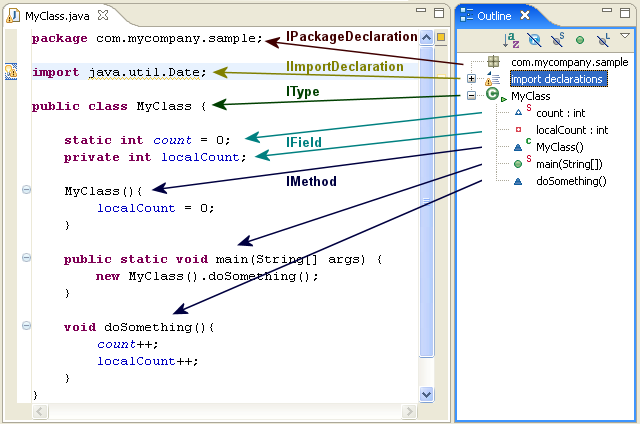
\includegraphics[width=\textwidth]{figures/javamodel2.png}
                \caption{Java Model elements from the source code}
                \label{fig:javamodel2.png}
        \end{subfigure}~
        \begin{subfigure}[b]{0.5\textwidth}
                \centering
                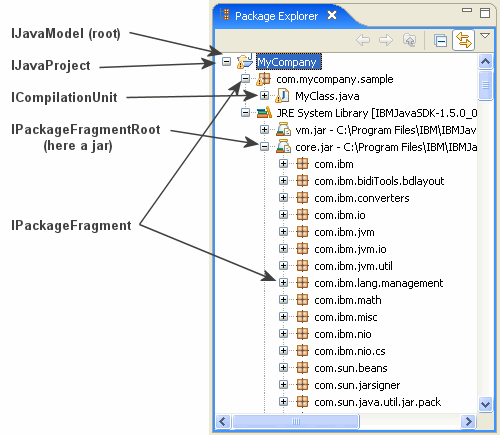
\includegraphics[width=\textwidth]{figures/javamodel1.png}
                \caption{Java Model elements from the navigator}
                \label{fig:javamodel1.png}
        \end{subfigure}
        \caption{Elements of the Java Model}\label{fig:javamodel}
\end{figure}
\autoref{fig:javamodel} (which comes from JDT's documentation) shows the
accessible interfaces if the Java model. Visible: literally every aspect 
is accessible from the projects down to method level.

Along numerous other features the plugin uses two specific ones:
subscription for model change:
\code{JavaCore.addElementChangedListener(IElementChangedListener);} static
method 
Search feature to resolve the dependency relationshisp between the elements.

The model change works: argument is a hierarchical delta with all the necessary infomration;
the implementations resp. to filter the information out.
We filter for the save methods.



\subsection{The generated EMF model}
\picr{wsmodel.pdf}{EMF model storing the structure of the Java projects}
\autoref{fig:wsmodel.pdf} shows the EMF model which is extracted and maintained from from the Java Model.

\subsection{The model synchronization process}

figure: > eclipse startup > gather all projects/classes/methods/relationships
and store them in the model.
Model change > filter > generate delta model > compare and merge emf subtrees.

Note: filter for save modifications, don't want to handle the incoherent working copy states. 


\section{Dependency data synchronizer}
RMI interface.
model queries.
Load workspace model.
Compact repository model.
 

\section{Model Query}

\subsection{Direct queries}
Explain the process how the direct queries go.
1-1 in the original documentation

\subsection{Pattern matching}
USing incquery to load models. To find dependencies. execute a set of matches.
Every time a workspace changes the result is updated.
Show the queries. What are they doing.
Join patterns.

Incoming queries. 
Impact analysis.



\section{UI Components}
How the user accesses to the  plugin

Input: user contributions.

Input: user saves the data > jdt propagates event to the source code moodel synchronizer.



\chapter{Evaluation}
%------------------------------------------------------------------------------
%3-4 pages. Functional evaluation. Performance evaluation. 
%------------------------------------------------------------------------------

\section{Example revisited}
Show how the tool solves the problem. Go through all components, show all
results one by one, what is the input and the output.
focus on the process again; show how each components work and put there the results, what would be seen.

\subsection{Dependency analysis}

Use: case binary repository filled with three jars
service
client
impl

Bytecode analysis. found statistics.
3  projects
8  classes
19 methods: 
   12 defined
   6 constructor (from non-interface class)
   1 static initializer(<clinit>)
2  fields

Dependency processing:
CLASSUSAGE hu.bme.incquery.deps.example.consumer.Main ----> hu.bme.incquery.deps.example.client.BasicImplUtil
CLASSUSAGE hu.bme.incquery.deps.example.consumer.Main ----> hu.bme.incquery.deps.example.service.Services
CLASSUSAGE hu.bme.incquery.deps.example.consumer.Main ----> hu.bme.incquery.deps.example.service.Service
METHODCALL hu.bme.incquery.deps.example.consumer.Main#main(java.lang.String[]):void ----> hu.bme.incquery.deps.example.client.BasicImplUtil#registerImplementationAsDefault():void
METHODCALL hu.bme.incquery.deps.example.consumer.Main#main(java.lang.String[]):void ----> hu.bme.incquery.deps.example.service.Services#newInstance(java.lang.String):hu.bme.incquery.deps.example.service.Service
METHODCALL hu.bme.incquery.deps.example.consumer.Main#main(java.lang.String[]):void ----> hu.bme.incquery.deps.example.service.Service#serviceB():void
CLASSINHER hu.bme.incquery.deps.example.client.BasicProvider ----> hu.bme.incquery.deps.example.service.Provider
CLASSUSAGE hu.bme.incquery.deps.example.client.BasicProvider ----> hu.bme.incquery.deps.example.service.Provider
CLASSUSAGE hu.bme.incquery.deps.example.client.BasicImplUtil ----> hu.bme.incquery.deps.example.service.Services
METHODCALL hu.bme.incquery.deps.example.client.BasicImplUtil#registerImplementation():void ----> hu.bme.incquery.deps.example.service.Services#registerProvider(java.lang.String,hu.bme.incquery.deps.example.service.Provider):void
METHODCALL hu.bme.incquery.deps.example.client.BasicImplUtil#registerImplementationAsDefault():void ----> hu.bme.incquery.deps.example.service.Services#registerProvider(java.lang.String,hu.bme.incquery.deps.example.service.Provider):void
FIELDREFER hu.bme.incquery.deps.example.client.BasicImplUtil#registerImplementationAsDefault():void ----> hu.bme.incquery.deps.example.service.Services.DEFAULT\_PROVIDER\_NAME
FIELDREFER hu.bme.incquery.deps.example.client.BasicImplUtil#registerImplementationAsDefault():void ----> hu.bme.incquery.deps.example.service.Services.DEFAULT\_PROVIDER\_NAME
CLASSINHER hu.bme.incquery.deps.example.client.BasicService ----> hu.bme.incquery.deps.example.service.AbstractService
CLASSUSAGE hu.bme.incquery.deps.example.client.BasicService ----> hu.bme.incquery.deps.example.service.AbstractService
METHODCALL hu.bme.incquery.deps.example.client.BasicService#BasicService():void ----> hu.bme.incquery.deps.example.service.AbstractService#AbstractService():void
METHODOVER hu.bme.incquery.deps.example.client.BasicService#serviceB():void ----> hu.bme.incquery.deps.example.service.AbstractService#serviceB():void
 
direct queries
compact  model
pattern matcher mechanism
results

\section{Performance evaluation}
Pure measurement. What can we measure:
the size of the database.
Speed of dependency discovery.
Size size of the compacted model. 
Memory size
\chapter{Conclusions and future work}
%------------------------------------------------------------------------------
%1 page. Evident content.
%------------------------------------------------------------------------------


\section{Results of the report}

In this paper we proposed an effective dependency analysis approach for
supporting smooth upgrades in large Java software infrastructure consisting of
tens of thousands of classes. It is based on a two-tiered approach, where the
server side is responsible for accumulating, storing and processing the incoming
dependency relations between the different API elements of the complete software
infrastructure, while the client side supports the developer by providing
instantaneous feedback on the dependency relations between the software modules
currently under development and the overall software infrastructure.

As a summary, my results in this work are the following:
\begin{itemize}
\item I designed a \emph{client-server based architecture for incoming
dependency analysis} of large Java software infrastructures.
\item I developed a \emph{binary dependency discovery module} for finding
dependencies between API elements within JARs.
\item I implemented a \emph{storage system} for the dependency relations and an
access layer for querying the dependency information.
\item I proposed a \emph{model-based dependency representation} based on EMF for
capturing local and remote dependencies.
\item I defined an \emph{incremental AST processing module} for discovering
source dependencies in the local workspace.
\item I implemented an \emph{on-the-fly dependency query engine} using
EMF-IncQuery for instantaneous dependency analysis feedback.
\item Finally, I evaluated the approach on the \emph{complete Java software
infrastructure at CERN} consisting of more than 1300 separate JARs.
\end{itemize}

%The \ptool{} is now a complete solution both with the explicit queries and its
%EMF-IncQuery-based extension. 

%The tool can be useful for a Java library developer who works at a large,
%software-oriented organization where lots of inter-depending softwares are
% developed and maintained and where binary compatibility and smooth upgrades are
% mission-critical requirements.
% 
% Both parts proved useful, fast and scalable enough for adaptation. EMF-IncQuery 
% showed that it can be applied to a specific domain and can be a useful core
% for fast model queries. 

\paragraph*{Application of the results}
As a major achievement, the server side modules of the porposed approach are
already used in production at CERN and its client side extension is also being
considered to be included in the upcoming release of the \ptool.

\section{Future work}
As of the future plans, there are plenty of directions to extend the
capabilities of the approach:
\begin{itemize}
\item In order to provide a better user notification on the client side we plan
to create a dedicated UI for highlighting the result of the local dependency
analysis. As Eclipse already provides a facility for searching for cross
compilation unit references, it is a straightforward task to integrate the model
queries there. Additionally, due to the instantaneous evaluation performance,
dependency analysis results could be displayed to the user as warnings or even
errors (supported by inline markers in Eclipse's source code editors) that
appear on-the-fly as the user is making a change that potentially violates
smooth upgrade policies.

%\item on-the-fly evaluated validation rules for instantaneous ``smooth upgrade" policy violation feedback

\item The second plan can be an extension for source-analysing not just Java,
but C++ programs too. We could make use of the capabilities of the Eclipse CDT
to provide AST support.

\item As a future improvement, we plan to support the definition of query-based
software metrics and use our on-the-fly query evaluation engine to enforce these
policies directly on the AST models.

\item Finally, an additional step forward would be the use of dynamic dependency
analysis techniques such as symbolic execution traces that would provide more
detailed dependecy information between the methods of the various modules.
\end{itemize}

%\addcontentsline{toc}{chapter}{Irodalomjegyzék}
%\bibliographystyle{plain}
%\bibliography{mybib}


%\include{appendices}

\label{page:last}
\end{document}
